\section{base64}
base64是一种用64个字符来表示任意二进制数据的方法。

用记事本打开exe,jpg,pdf这些文件时,我们都会看到一大堆乱码。因为二进制文件包含很多无法显示和打印的字符,所以如果要让记事本这样额的文本处理软件处理二进制数据,就需要一个二进制到字符串的转换方法。Base64是一种最常见的二进制编码方法。

Base64的原理很简单,首先,准备一个包含64个字符串的数组:
['A','B','C',\ldots,'a','b','c',\ldots,'0','1',\ldots,'+','/']

然后对二进制数据进行处理,每3个字节一组,一共是$3\times8=24bit$,划为4组,每组正好6个bit。
\begin{figure}[H]
	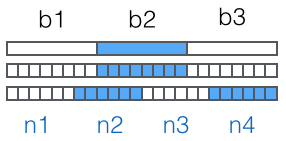
\includegraphics{base64.png}
\end{figure}
这样我们得到4个数字所谓索引,然后查表,获得相应的4个字符,这就是编码后的字符串。所以Base64编码会把3字节的二进制数据编码为4字节的文本数据,长度正佳33\%。好处是编码后的文本数据可以在邮件正文,网页等直接显示。

如果需要编码的二进制数据不是3的倍数,最后会剩下1个或2个字节怎么办?Base64用\\x00字节在末尾补足后,再在编码的末尾加上一个或者2个=号,表死补了多少字节,解码的时候会自动去掉。

python内置的base64可以直接进行base64编码解码:
\begin{python}
In [15]: import base64
In [17]: base64.b64encode(b'binary\x00string')
Out[17]: b'YmluYXJ5AHN0cmluZw=='
In [18]: ben = base64.b64encode(b'binary\x00string')
In [19]: base64.b64decode(ben)
Out[19]: b'binary\x00string'
In [20]: ben
Out[20]: b'YmluYXJ5AHN0cmluZw=='
\end{python}
由于标准的base64编码后可能出现+和/。在URL中就不能直接作为参数,所以又有之中"url safe"的base64编码,其实就是吧字符+和/分别变成了-和\_。
\begin{python}
In [23]: base64.b64encode(b'i\xb7\x1d\xfb\xef\xff')
Out[23]: b'abcd++//'
In [25]: bus = base64.urlsafe_b64encode(b'i\xb7\x1d\xfb\xef\xff')
In [26]: base64.urlsafe_b64decode(bus)
Out[26]: b'i\xb7\x1d\xfb\xef\xff'
In [27]: bus
Out[27]: b'abcd--__'
\end{python}

Base64是一同通过查表的编码方法,不能用于加密,即使使用自定义的编码表也不行。

Base64适用于小段内容的编码,比如数字证书签名,Cookie的内容等。

由于=字符也可能出现在Base64编码中,但=用在URL,Cookie里面会造成歧义,所以很多Base64编码后会把=去掉:
\begin{python}
# 标准Base64:
'abcd' -> 'YWJjZA=='
# 自动去掉=:
'abcd' -> 'YWJjZA'
\end{python}
去掉=后怎么解码呢?因为Base64是把3个字节变成4个字节,所以,Base64编码的长度永远是4的倍数,因此,需要加上=吧Base64字符串长度变为4的倍数就可以正常解码了。
